%% LaTeX-Beamer template for KIT design
%% by Erik Burger, Christian Hammer
%% title picture by Klaus Krogmann
%%
%% version 2.0
%%
%% mostly compatible to KIT corporate design v2.0
%% http://intranet.kit.edu/gestaltungsrichtlinien.php
%%
%% Problems, bugs and comments to
%% burger@kit.edu

\documentclass[18pt]{beamer}
\usetheme{kit}

%% TITLE PICTURE

% if a custom picture is to be used on the title page, copy it into the 'logos'
% directory, in the line below, replace 'mypicture' with the 
% filename (without extension) and uncomment the following line
% (picture proportions: 63 : 20, *.eps format if you use latex+dvips+ps2pdf,
% *.jpg/*.png/*.pdf if you use pdflatex)

%\titleimage{mypicture}

%% TITLE LOGO

% for a custom logo on the front page, copy your file into the 'logos'
% directory, insert the filename in the line below and uncomment it

%\titlelogo{mylogo}

% (*.eps format if you use latex+dvips+ps2pdf,
% *.jpg/*.png/*.pdf if you use pdflatex)

%% BIBTEX ICON/KEY

% if you want to see BibTeX keys in the references view instead of the symbol,
% uncomment the following line
% \usebibitemtemplate{\insertbiblabel}

% the presentation starts here

% change the following line to "ngerman" for German style date and logos
% change the following line to "english" for English style date and logos
\selectlanguage{ngerman}

\beamertemplatenavigationsymbolsempty

\usepackage{listings}
\definecolor{darkgray}{rgb}{0.95,0.95,0.95}
\definecolor{darkgreen}{rgb}{0.05,0.7,0.05}
\lstset{ language=Java,
	backgroundcolor=\color{darkgray}, 
	numbers=none, 
	keywordstyle=\color{black}\bfseries,
	tabsize=2,
	showspaces=false,               % show spaces adding particular underscores
	showstringspaces=false,         % underline spaces within strings
	showtabs=false, 
}



\title[Tutorium06]{Tutorium 06: Parallelismus und Testen}
\subtitle{Softwaretechnik im SS 2011, Tutorium 4}
\author{Jürgen Walter}
\date{\today}

\institute{Chair for Software Design and Quality}

\begin{document}

%title page
\begin{frame}
\titlepage
\end{frame}

%table of contents
\frame{
\frametitle{Was machen wir heute?}
	\tableofcontents
}

\section{Rückblick}

\frame{
\frametitle{Rückblick ÜB6}

	\begin{block}{Aufgabe 1 - Kontrollflussorientiertes Testen}
	\begin{itemize}
	\item kommt oft in der Klausur vor \pause
	\item relativ leicht verdiente Punkte!
	\end{itemize}
	\end{block}
}

\frame{
\frametitle{Rückblick ÜB6}

	\begin{block}{Aufgabe 2 -Gebietszerlegung und Synchronisation}
	\begin{itemize} \pause
	\item a) sollte jeder hinbekommen - falls euch nichts einfällt wählt einfach ein paar Parameter und schaut was passiert \pause
	\item b) sieht auf den ersten Blick harmlos aus - um sicher zu gehen programmiert ein Testprogramm und testet, ob euer Fix tatsächlich das Problem behebt \pause
	\item stellt dazu auch sicher, dass die ursprüngliche Barriere tatsächlich falsch funktioniert in eurem Test-Programm \pause
	\item ein Test ist nur dann sinnvoll, wenn er den Unterschied zwischen richtigem und falschem Code auch zeigt - \pause
	\item sonst kann es sein, dass euer Test das eigentliche Fehlverhalten nicht sichtbar macht \pause
	\item Achtung: wait() kann auch ``grundlos'' enden, daher sollte wait() immer in einer Schleife stehen
	\end{itemize}
	\end{block}
}


\frame{
\frametitle{Rückblick ÜB6}
	\begin{block}{Aufgabe 3 - Parallelisierung}
	\begin{itemize}
	\item für diese Aufgabe gibt es 9 ``Pflicht''- und 5 Bonuspunkte
	\item ihr braucht zum Testen einen Rechner mit mindestens zwei Kernen - \\
		falls ihr keinen habt, gibt es in der Atis genug davon (Core2Duo, Core i5, Athlon X2)
	\item zuverlässige Laufzeitmessungen kann man oft brauchen, und es gibt dabei mehr als genug Fehlerquellen ;-) \pause
	\item Zeitmessungen sind immer ungenau - die Bearbeitungszeit sollte daher nicht kürzer als eine Sekunde sein \pause
	\item das Programm soll sowohl: \\
		mit Kommandozeilenargumenten mit Hilfe von Configuration.java (wie bei ÜB2), \\ \pause
		also auch ohne Argumente mit einem GUI (wie bei ÜB3) gestartet werden können
	\end{itemize}
	\end{block}
}

\section{Zum Aufwärmen}

\frame {
\frametitle{Wahr oder falsch?}
\begin{itemize}
	\color<2->[rgb]{1,0,0}
	\item Die letzte Phase des klassischen Wasserfallmodells ist „Testen und Abnahme“.
	\color[rgb]{0,0,0}
	\pause
	\color<3->[rgb]{0,1,0}
	\item Regressionstests helfen verhindern, dass alte Fehler wieder auftreten.
	\color[rgb]{0,0,0}
	
	\pause
	\color<4->[rgb]{1,0,0}
	\item Funktionale Attribute spezifizieren wie gut die Software ihre Funktionen erfüllt.
	\color[rgb]{0,0,0}
	\pause
	\color<5->[rgb]{0,1,0}
	\item Bei Gleichheit 0. Stufe handelt es sich um identische Objekte.
	\color[rgb]{0,0,0}
	\pause
	\color<6->[rgb]{1,0,0}
	\item In einer transparenten Schichtenarchitektur kann eine Schicht sowohl auf die nächsthöhere als auch die nächstniedrigere Schicht zugreifen
	\color[rgb]{0,0,0}
	\pause
	\color<7->[rgb]{1,0,0}
	\item Bei der Anforderungsvalidierung in der Planungsphase wird nicht überprüft, ob die Anforderungen erfüllt werden können.
	\color[rgb]{0,0,0}


\end{itemize}
}

\frame {
\frametitle {Klausuraufgaben zum Aufwärmen} 
	\begin{block} {Aufgabe 1 (1P)}
	Was ist der Nachteil von Zyklen in der Benutzt-Relation zwischen Modulen?\\
	\begin{itemize}
		\visible<2-> {
		\item Die einzelnen Module können nicht nacheinander implementiert
			und getestet werden, weil ihr Funktionieren von einer korrekten
			Implementierung aller Module des Zyklus abhängt.
		\item Oder: „Nothing works until everything works.“
		}
	\end{itemize}
	\end{block}
}

\frame {
\frametitle {Klausuraufgaben zum Aufwärmen} 
	\begin{block} {Aufgabe 2 (2P)}
		Nennen Sie jeweils zwei in der Vorlesung besprochene Entwurfsmuster der Kategorien 						Entkopplungsmuster und Variantenmuster und ordnen Sie die genannten Entwurfsmuster der 					entsprechenden Kategorie zu. \\
		\begin{itemize}
			\item Entkopplungsmuster: 
			\visible<2-> {Adapter, Beobachter, Brücke, Iterator, Stellvertreter, Vermittler}
			\item Variantenmuster:
			\visible<3-> {Abstrakte Fabrik, Besucher, Erbauer, Fabrikmethode, Kompositum, 						Schablonenmethode, Strategie, Dekorierer}
		\end{itemize}
	\end{block}
}


\section{Klausur-Tipps}

\frame {
\frametitle{Aufgabe a)}

a) Übersetzen sie den Algorithmus in die in der Vorlesung besprochene Zwischensprache und erstellen sie daraus den Kontrollflussgraphen
\begin{center}
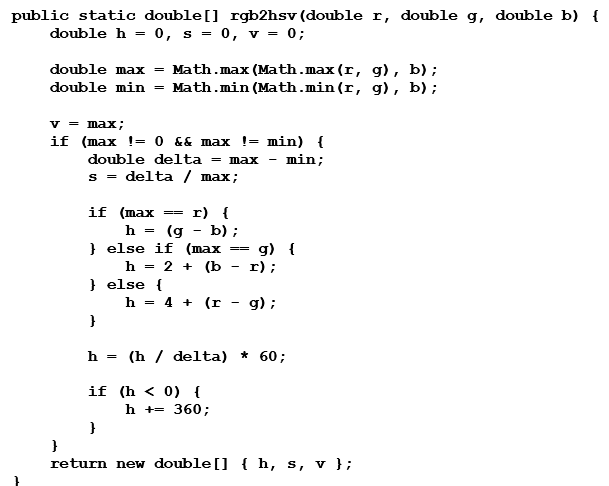
\includegraphics[scale=0.45]{pics/05/code.png}
\end{center}

}

\begin{frame}[fragile]
\frametitle {Klausuraufgabe} 
	\begin{block} {Aufgabe (1P)}

	\begin{lstlisting} {}
	public static double blub(double[] d) {
		if  (d != null && d.length > 0) {
		...
		}
		...
	}
	\end{lstlisting}
	Begründen Sie: Was wäre die Folge, wenn man das \&\& durch ein \& ersetzt?

	\begin{itemize}	
	\visible<2-> {
	\item Keine Kurzauswertung (0,5 P) 
	\item $\Rightarrow$ Bei null als Eingabe gäbe es eine NullPointerExeption bei d.length (0,5 P).
	}
	\end{itemize}
	\end{block} 
\end{frame}


\section{Ende}

\frame{
\frametitle{Viel Erfolg!}

	\begin{block}{Aufgabe 1 - Kontrollflussorientiertes Testen}
	\begin{itemize}
	\item kommt oft in der Klausur vor \pause
	\item relativ leicht verdiente Punkte!
	\end{itemize}
	\end{block}
}


\frame{
\frametitle{Bis zum nächsten Mal}
	\begin{center}
	
\includegraphics[height=200pt]{pics/06/06_comic}
	\end{center}
}

\end{document}
